% 
% MASTER'S LEVEL COMPUTER VISION PRESENTATION
% Testing with Out-of-Sample Data: A Deep Dive into Generalization
% Student: Davar Adil Yassin | UKH | Instructor: Dr. Polla
% ============================================================================

\documentclass[aspectratio=169,10pt]{beamer}

% THEME & PACKAGES
\usetheme{metropolis}
\usepackage{graphicx}
\usepackage{tikz}
\usetikzlibrary{positioning,shapes,arrows,calc,backgrounds,fit,decorations.pathreplacing}
\usepackage{amsmath,amsfonts,amssymb}
\usepackage{hyperref}
\usepackage{booktabs}
\usepackage{bm}
\usepackage{colortbl}
\usepackage{algorithm}
\usepackage{algpseudocode}
\usepackage{multirow}
\usepackage{xcolor}
\usepackage{tcolorbox}
\graphicspath{{Images/}}

% COLORS
\definecolor{ukhblue}{RGB}{0,51,102}
\definecolor{ukhlight}{RGB}{0,110,180}
\definecolor{alertred}{RGB}{204,0,0}
\definecolor{successgreen}{RGB}{0,128,0}
\definecolor{warningorange}{RGB}{255,140,0}

% BEAMER COLOR CUSTOMIZATION
\setbeamercolor{title}{fg=ukhblue}
\setbeamercolor{frametitle}{fg=white}
\setbeamercolor{progress bar}{fg=ukhblue,bg=gray!20}
\setbeamercolor{palette primary}{bg=ukhblue, fg=white}
\setbeamercolor{palette secondary}{bg=ukhlight, fg=white}
\setbeamercolor{structure}{fg=ukhblue}
\setbeamercolor{block title}{bg=ukhblue,fg=white}
\setbeamercolor{block body}{bg=gray!10}

% CUSTOM BOXES
\newtcolorbox{keypoint}{colback=ukhlight!10,colframe=ukhlight,title=Key Point}
\newtcolorbox{warning}{colback=warningorange!10,colframe=warningorange,title=Common Pitfall}
\newtcolorbox{reality}{colback=alertred!10,colframe=alertred,title=Reality Check}
\newtcolorbox{philosophical}{colback=gray!5,colframe=gray!50,title=Philosophical Reflection}

% FOOTER
\setbeamertemplate{footline}{
  \leavevmode%
  \hbox{%
  \begin{beamercolorbox}[wd=.5\paperwidth,ht=2.5ex,dp=1ex,left]{author in head/foot}%
    \hspace*{1em}\usebeamerfont{author in head/foot}%
    Davar Adil Yassin \quad—\quad UKH \quad—\quad Computer Vision (MSc AI)
  \end{beamercolorbox}%
  \begin{beamercolorbox}[wd=.25\paperwidth,ht=2.5ex,dp=1ex,center]{date in head/foot}%
    \usebeamerfont{date in head/foot}\today
  \end{beamercolorbox}%
  \begin{beamercolorbox}[wd=.25\paperwidth,ht=2.5ex,dp=1ex,right]{date in head/foot}%
    \usebeamerfont{date in head/foot}\insertframenumber{} / \inserttotalframenumber\hspace*{1em}
  \end{beamercolorbox}}%
  \vskip0pt%
}
\setbeamertemplate{navigation symbols}{}

% TITLE INFORMATION
\title{Testing with Out-of-Sample Data}
\subtitle{Why Data is the new Gold?}
\author{Davar Adil Yassin}
\institute{
    University of Kurdistan Hewlêr (UKH)\\
    Master's in Artificial Intelligence\\
    Computer Vision\\[0.5em]
    \textit{Instructor: Dr. Polla Fattah}
}
\titlegraphic{\hfill\includegraphics[height=1.5cm]{UKH_logo.png}}
\date{\today}

\begin{document}

% ============================================================================
% TITLE & OPENING
% ============================================================================

\begin{frame}
  \titlepage
\end{frame}

\begin{frame}{Data: The New Gold}
\begin{philosophical}
\small
\textit{"The most important asset in the modern world is not oil, not gold, not even land—it is data."}\\
\hfill —Yuval Noah Harari, \textit{Homo Deus}
\end{philosophical}

\vspace{0.4em}

\textbf{Three centuries ago:}
\begin{itemize}
    \setlength{\itemsep}{0.15em}
    \small
    \item Industrial Revolution: coal and oil
    \item Power from physical resources
\end{itemize}

\vspace{0.3em}

\textbf{Today:}
\begin{itemize}
    \setlength{\itemsep}{0.15em}
    \small
    \item Information Revolution: \textbf{data}
    \item Power from understanding data
\end{itemize}

\vspace{0.4em}

\begin{alertblock}{The Paradox}
\small More data than ever, yet most fail to extract wisdom.
\end{alertblock}
\end{frame}



\begin{frame}{Why Harari Matters Here}
\small
\textbf{Yuval Noah Harari's key works:}

\begin{description}
  \small
  \item[\textit{Homo Deus} (2015)] Data and algorithms reshaping civilization. Introduces \textbf{dataism}.
  \item[\textit{Nexus} (2024)] Information flows and how networks shape societies and AI.
\end{description}

\vspace{0.5em}

\textbf{Why we reference him:}
\begin{itemize}
    \setlength{\itemsep}{0.15em}
    \small
    \item Frames data as a philosophical revolution
    \item Connects technical work to deeper questions about AI
\end{itemize}
\end{frame}

\begin{frame}{Opening: The Illusion of Intelligence}
\begin{philosophical}
\textit{"In the age of information, the scarcest resource is not information itself, but the wisdom to know what information matters."}\\
\hfill — Yuval Noah Harari, \textit{Nexus}
\end{philosophical}

\vspace{1em}

\textbf{Today's journey:}
\begin{itemize}
    \item We train models on data — but do they \textbf{understand} or merely \textbf{memorize}?
    \item We achieve 98\% accuracy — but what does that \textit{really} mean?
    \item We deploy AI systems — but do they work when the world changes?
\end{itemize}

\vspace{0.5em}
This lecture goes far beyond Chapter 11 of \textit{Neural Networks From Scratch}. We explore the philosophical, mathematical, and practical depths of generalization.
\end{frame}

\begin{frame}[fragile]{Outline}
\small
\setlength{\leftmargini}{1.0cm}
\begin{itemize}
    \setlength{\itemsep}{0.35em}
    \item \textbf{Foundations} — Why Generalization Matters
    \item \textbf{Data Splitting} — The Foundation of Honest Evaluation
    \item \textbf{Data Leakage} — The Silent Killer
    \item \textbf{Evaluation Metrics} — Beyond Accuracy
    \item \textbf{Bias-Variance Tradeoff} and Generalization Theory
    \item \textbf{Distribution Shift} — When the World Changes
    \item \textbf{Dataset Bias} and Shortcut Learning
    \item \textbf{Overfitting and Regularization}
    \item \textbf{Case Studies} — Real-World Failures
    \item \textbf{Practical Checklist} and Best Practices
    \item \textbf{Philosophical Reflections} and Future
\end{itemize}

\vspace{0.6em}

\begin{center}
\colorbox{ukhblue!15}{%
  \parbox{0.85\textwidth}{
    \small
  }
}
\end{center}
\end{frame}

% ============================================================================
\section{Foundations — Why Generalization Matters}
% ============================================================================

\begin{frame}
\begin{philosophical}
\textit{"Believing that more information is always good is like believing that more food is always good. We should be careful with what we put in our mind, not just our body — is it time for an information diet?"}\\\hfill — Yuval Noah Harari
\end{philosophical}
\end{frame}

\begin{frame}{The Central Question of Machine Learning}
\begin{center}
\Large \textbf{Can our model perform well on data it has never seen?}
\end{center}

\vspace{1em}

\begin{columns}
\column{0.48\textwidth}
\textbf{Training Performance:}
\begin{itemize}
    \item Easy to achieve
    \item Can be 100\% with enough capacity
    \item Tells us almost nothing
\end{itemize}

\column{0.48\textwidth}
\textbf{Real-World Performance:}
\begin{itemize}
    \item Hard to predict
    \item Subject to distribution shift
    \item \alert{This is what matters}
\end{itemize}
\end{columns}

\vspace{1em}
\begin{reality}
Most AI failures occur not in the lab, but in deployment — on new cameras, new populations, new lighting conditions, new contexts.
\end{reality}
\end{frame}

\begin{frame}
\begin{philosophical}
\small
\textit{"We are now creating tame humans that produce enormous amounts of data and function as very efficient chips in a huge data-processing mechanism, but these data-cows hardly maximize the human potential. If we are not careful, we will end up with downgraded humans misusing upgraded computers to wreak havoc on themselves and on the world."}\\\hfill — Yuval Noah Harari
\end{philosophical}
\end{frame}

\begin{frame}{Analogy: The Two Students}
\begin{center}
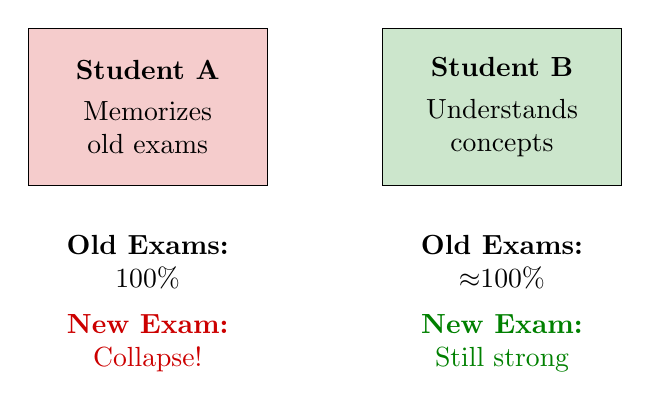
\begin{tikzpicture}[scale=0.9]
    % Student A
    \node[draw,rectangle,minimum width=3cm,minimum height=2cm,fill=alertred!20] (A) at (0,0) {
        \begin{minipage}{2.8cm}
        \centering
        \textbf{Student A}\\[0.3em]
        Memorizes\\
        old exams
        \end{minipage}
    };
    
    % Student B
    \node[draw,rectangle,minimum width=3cm,minimum height=2cm,fill=successgreen!20] (B) at (5,0) {
        \begin{minipage}{2.8cm}
        \centering
        \textbf{Student B}\\[0.3em]
        Understands\\
        concepts
        \end{minipage}
    };
    
    % Old exam results
    \node[below=0.5cm of A,align=center] {\textbf{Old Exams:}\\100\%};
    \node[below=0.5cm of B,align=center] {\textbf{Old Exams:}\\$\approx$100\%};
    
    % New exam results
    \node[below=1.5cm of A,align=center,text=alertred] {\textbf{New Exam:}\\Collapse!};
    \node[below=1.5cm of B,align=center,text=successgreen] {\textbf{New Exam:}\\Still strong};
\end{tikzpicture}
\end{center}

\textbf{Neural networks are naturally Student A.}\\
Our job: make them more like Student B.
\end{frame}



\begin{frame}{From Chapter 11: The Spiral Dataset Warning}
The book shows us:
\begin{itemize}
    \item Training accuracy: 98.3\%
    \item Test accuracy: 80.3\%
    \item Training loss: 0.074
    \item Test loss: 0.858
\end{itemize}

\vspace{1em}

\begin{warning}
This 18\% gap is \textbf{not} a small detail — it reveals fundamental overfitting. The model memorized noise instead of learning the underlying function.
\end{warning}

\vspace{0.5em}
We will dissect \textit{why} this happens, \textit{how} to detect it, and \textit{what} to do about it.
\end{frame}


% ============================================================================
\section{Data Splitting — The Foundation of Honest Evaluation}
% ============================================================================

\begin{frame}{Why Split Data? The Philosophical Answer}
\begin{philosophical}
\textit{"The most dangerous lies are the ones we tell ourselves."}\\
\hfill — Harari on human self-deception
\end{philosophical}

\vspace{1em}

If we evaluate a model only on training data:
\begin{itemize}
    \item We are \textbf{lying to ourselves} about its capabilities
    \item We create an \textbf{illusion of intelligence}
    \item We will face catastrophic failure in deployment
\end{itemize}

\vspace{0.5em}
Data splitting is our defense against self-deception.
\end{frame}

\begin{frame}{The Three-Way Split: Train / Validation / Test}
\begin{center}
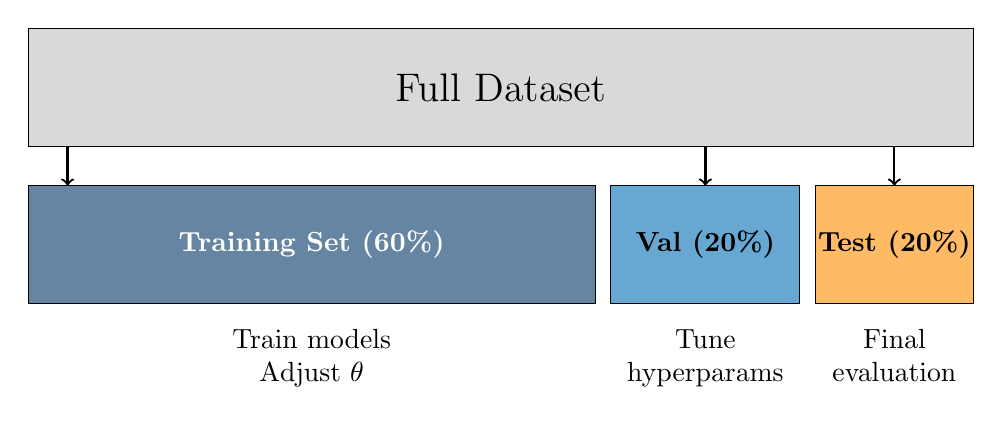
\begin{tikzpicture}[scale=1]
    % Full dataset
    \draw[fill=gray!30] (0,0) rectangle (12,1.5);
    \node at (6,0.75) {\Large Full Dataset};
    
    % Split boxes
    \draw[fill=ukhblue!60] (0,-2) rectangle (7.2,-0.5);
    \node[white] at (3.6,-1.25) {\textbf{Training Set (60\%)}};
    
    \draw[fill=ukhlight!60] (7.4,-2) rectangle (9.8,-0.5);
    \node at (8.6,-1.25) {\textbf{Val (20\%)}};
    
    \draw[fill=warningorange!60] (10,-2) rectangle (12,-0.5);
    \node at (11,-1.25) {\textbf{Test (20\%)}};
    
    % Arrows
    \draw[->,thick] (0.5,0) -- (0.5,-0.5);
    \draw[->,thick] (8.6,0) -- (8.6,-0.5);
    \draw[->,thick] (11,0) -- (11,-0.5);
    
    % Usage labels
    \node[below,align=center] at (3.6,-2.2) {Train models\\Adjust $\theta$};
    \node[below,align=center] at (8.6,-2.2) {Tune\\hyperparams};
    \node[below,align=center] at (11,-2.2) {Final\\evaluation};
\end{tikzpicture}
\end{center}

\begin{keypoint}
Validation $\neq$ Test! Validation is used iteratively during development. Test is \textbf{only touched once}, at the very end.
\end{keypoint}
\end{frame}

\begin{frame}{Validation Set: Your Development Compass}
\textbf{Purpose of validation set:}
\begin{itemize}
    \item Tune learning rate, weight decay, dropout rate
    \item Choose architecture (number of layers, neurons)
    \item Decide when to stop training (early stopping)
    \item Compare different model variants
\end{itemize}

\vspace{1em}

\textbf{Analogy:} Validation set = practice exams before the final\\
You can take them many times, adjust your study strategy, learn from mistakes.

\vspace{0.5em}

\begin{warning}
Every time you use validation performance to make a decision, you leak a tiny bit of information. This is unavoidable but must be managed carefully.
\end{warning}
\end{frame}

\begin{frame}{Test Set: The Moment of Truth}
\textbf{Purpose of test set:}
\begin{itemize}
    \item Provide an \textbf{unbiased} estimate of final performance
    \item Evaluate generalization to truly unseen data
    \item Report to stakeholders, publish in papers
\end{itemize}

\vspace{1em}

\textbf{Golden rules:}
\begin{enumerate}
    \item Never train on test data (obviously!)
    \item Never tune hyperparameters based on test performance
    \item Ideally, evaluate test set \textbf{only once}
    \item If you must evaluate multiple times, be transparent about it
\end{enumerate}

\vspace{0.5em}

\textbf{Analogy:} Test set = the actual final exam\\
You get one shot. Your score represents your true capability.
\end{frame}

\begin{frame}{Common Splitting Ratios}
\begin{table}
\centering
\begin{tabular}{lccc}
\toprule
\textbf{Dataset Size} & \textbf{Train} & \textbf{Val} & \textbf{Test} \\
\midrule
Small ($<10k$) & 60\% & 20\% & 20\% \\
Medium ($10k$--$100k$) & 70\% & 15\% & 15\% \\
Large ($100k$--$1M$) & 80\% & 10\% & 10\% \\
Very large ($>1M$) & 90\%+ & 5\% & 5\% \\
\bottomrule
\end{tabular}
\end{table}

\vspace{1em}

\textbf{Principle:} As dataset grows, you need fewer samples for reliable validation/test estimates.

\vspace{0.5em}

Example: With 1M samples, even 5\% = 50,000 test samples (more than enough for robust evaluation).
\end{frame}

\begin{frame}{Computer Vision: Beware of Hidden Correlations}
Similar issues arise in Computer Vision:

\vspace{0.5em}

\begin{tabular}{l|p{6cm}}
\toprule
\textbf{Problem} & \textbf{Solution} \\
\midrule
Same patient in train/test & Split by \textbf{patient ID}, not by image \\
Video frames & Split by \textbf{video sequence}, not frame \\
Same scene, different angles & Split by \textbf{scene/location} \\
Medical: same hospital & Split by \textbf{institution} if possible \\
\bottomrule
\end{tabular}

\vspace{1em}

\begin{keypoint}
Always ask: \textit{"What is the fundamental unit that should not be split?"} Define the splitting unit, then split at that level.
\end{keypoint}
\end{frame}

% ============================================================================
\section{Data Leakage — The Silent Killer}
% ============================================================================

\begin{frame}{What is Data Leakage?}
\textbf{Definition:} Information from outside the training set "leaks" into the model, artificially inflating performance estimates.

\vspace{1em}

\textbf{Why it's dangerous:}
\begin{itemize}
    \item Creates illusion of high accuracy
    \item Model appears to generalize but doesn't
    \item Discovered only after deployment failure
\end{itemize}

\vspace{1em}

\begin{reality}
According to Kaggle surveys, data leakage is one of the top reasons competition winners' models fail in production.
\end{reality}
\end{frame}

\begin{frame}[fragile]{Analogy: The Exam Cheat Sheet}
\begin{center}
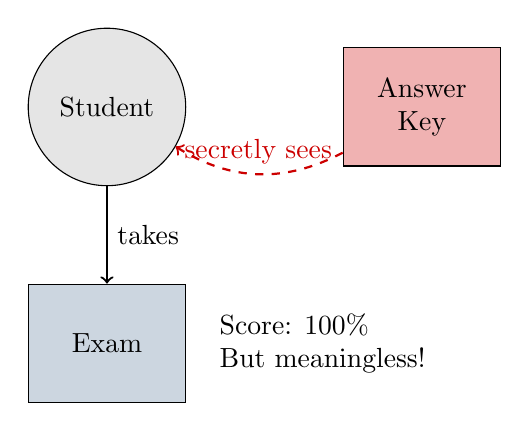
\begin{tikzpicture}[node distance=2cm]
    % Student
    \node[draw,circle,minimum size=2cm,fill=gray!20] (student) at (0,0) {Student};
    
    % Answer key
    \node[draw,rectangle,fill=alertred!30,minimum width=2cm,minimum height=1.5cm,align=center] (answers) at (4,0) {Answer\\Key};
    
    % Arrow with "secretly sees"
    \draw[->,thick,alertred,dashed] (answers) to[bend left=30] node[above] {secretly sees} (student);
    
    % Exam
    \node[draw,rectangle,fill=ukhblue!20,minimum width=2cm,minimum height=1.5cm] (exam) at (0,-3) {Exam};
    
    % Takes exam arrow
    \draw[->,thick] (student) -- (exam) node[midway,right] {takes};
    
    % Score
    \node[right=0.3cm of exam,align=left] {Score: 100\%\\But meaningless!};
\end{tikzpicture}
\end{center}

\textbf{In ML:} Leakage = model secretly "seeing" test set characteristics during training.
\end{frame}

\begin{frame}{Data Leakage Problem 1: Duplicate Images}

\textbf{What happens:} The same image (or a slightly modified version) appears in both training and test sets.

\vspace{1em}

\textbf{Why it's a problem:}
\begin{itemize}
    \item Your model doesn't generalize — it just memorizes
    \item Test performance looks artificially high
    \item Real-world performance will be much worse
\end{itemize}

\vspace{1em}

\textbf{Example:}
\begin{itemize}
    \item You augment a training image (rotate, crop, flip)
    \item Same augmented version ends up in test set by accident
    \item Model "recognizes" it from training, but didn't actually learn anything new
\end{itemize}

\vspace{1em}

\textbf{Solution:} Use perceptual hashing to find near-duplicate images before splitting.
\end{frame}

\begin{frame}{Data Leakage Problem 2: Using Test Data by Accident}

\textbf{What happens:} You use information from your test set while building or tuning your model.

\vspace{1em}

\textbf{Why it's a problem:}
\begin{itemize}
    \item Your model learns the test data, not the real pattern
    \item Test performance is fake — artificially inflated
    \item Real-world performance will be much worse
\end{itemize}

\vspace{1em}

\textbf{Simple Example: Tuning hyperparameters}
\begin{itemize}
    \item You try 10 different learning rates
    \item You evaluate each one on your test set
    \item You pick the best performing learning rate
    \item But you've now \textit{tuned} your model to the test set!
    \item Test accuracy is no longer honest
\end{itemize}

\vspace{1em}

\textbf{Correct approach:} Use \textbf{validation set} to pick best hyperparameters. Only check test set \textbf{once}, at the very end.
\end{frame}

\begin{frame}{Data Leakage Problem 3: Temporal Leakage in Video}

\textbf{What happens:} Different frames from the same video are split randomly between train and test.

\vspace{1em}

\textbf{Why it's a problem:}
\begin{itemize}
    \item Consecutive video frames are highly similar
    \item If frame $t$ is in training and frame $t+1$ is in test, the model has seen almost the same content
    \item Test performance doesn't reflect real generalization
\end{itemize}

\vspace{1em}

\textbf{Example:}
\begin{itemize}
    \item Video sequence: 30 frames per second
    \item Frame 1–25 in training, Frame 26–30 in test
    \item If you randomly split, Frame 25 from training is nearly identical to Frame 26 in test
\end{itemize}

\vspace{1em}

\textbf{Solution:} Split by \textbf{entire video}, not individual frames.
\end{frame}

\begin{frame}{Data Leakage Problem 4: Label/Metadata Leakage}

\textbf{Simple explanation:} Your data accidentally reveals the answer.

\vspace{0.6em}

\textbf{Real example:}
\begin{itemize}
    \setlength{\itemsep}{0.2em}
    \small
    \item Task: Classify X-rays as "sick" or "healthy"
    \item Dataset has column: \texttt{hospital\_id}
    \item Hospital A = mostly sick patients, Hospital B = mostly healthy
    \item Model learns: \texttt{if hospital\_id == A $\rightarrow$ sick}
    \item Never looks at the actual X-ray!
\end{itemize}

\vspace{0.6em}

\textbf{Why dangerous:}
\begin{itemize}
    \setlength{\itemsep}{0.2em}
    \small
    \item 95\% accuracy in testing (looks amazing!)
    \item Deploy at new Hospital C: total failure
    \item Model can't read X-rays, only IDs
\end{itemize}

\vspace{0.5em}

\textbf{Fix:} Remove metadata columns like IDs, filenames, timestamps before training
\end{frame}


\begin{frame}{How to Prevent Leakage: Best Practices}
\small
\textbf{Golden Rule:} Test set is sacred. Touch it \textbf{only once} at the very end.

\vspace{0.4em}

\textbf{Safe workflow (in order):}

\vspace{0.3em}

\begin{enumerate}
    \setlength{\itemsep}{0.2em}
    \small
    \item \textbf{Split first:} Train/val/test \textit{before} any processing
    \item \textbf{Apply to validation:} Use training stats, tune hyperparameters
    \item \textbf{Final test:} Apply same preprocessing, evaluate once
\end{enumerate}

\vspace{0.4em}

\end{frame}


\begin{frame}{Detecting Leakage After the Fact}
\textbf{Red flags that suggest possible leakage:}

\begin{itemize}
    \item Test accuracy unrealistically close to train accuracy (e.g., both 99.8\%)
    \item Performance dramatically drops on external validation set
    \item Simple baseline (logistic regression) performs as well as deep model
    \item Feature importance shows suspicious variables (IDs, timestamps)
\end{itemize}

\vspace{1em}

\textbf{Diagnostic procedure:}
\begin{enumerate}
    \item Re-split data with different random seed — does performance stay stable?
    \item Remove suspicious features — does accuracy collapse?
    \item Test on completely external dataset — realistic performance?
\end{enumerate}
\end{frame}

% ============================================================================
\section{Evaluation Metrics — Beyond Accuracy}
% ============================================================================

\begin{frame}
\begin{center}
\Large
\textit{"A model can be accurate and still be unjust."}
\end{center}
\end{frame}

\begin{frame}{The Tyranny of Accuracy}
\small
\begin{reality}
\small
\textbf{Scenario:} Disease detection. Dataset: 99\% healthy, 1\% diseased.

A model predicting ``healthy'' for \textit{every} image gets 99\% accuracy but catches zero disease!
\end{reality}

\vspace{0.5em}

\textbf{Accuracy formula:}
\[
\text{Accuracy} = \frac{TP + TN}{TP + TN + FP + FN}
\]

\vspace{0.4em}

\textbf{\textcolor{successgreen}{When accuracy works:}} Balanced classes

\vspace{0.3em}

\textbf{\textcolor{alertred}{When accuracy fails:}}
\begin{itemize}
    \setlength{\itemsep}{0.1em}
    \small
    \item Imbalanced datasets (very common in CV)
\end{itemize}

\vspace{0.3em}

\small \textit{Better metrics: Precision, Recall, F1-score}
\end{frame}

\begin{frame}{The Confusion Matrix: Foundation of All Metrics}

\begin{center}
\begin{tabular}{c|c|c}
  & \textbf{Pred: Positive} & \textbf{Pred: Negative} \\
\hline
\textbf{Actual: Positive} & \cellcolor{successgreen!40}\textbf{TP} & \cellcolor{alertred!40}\textbf{FN} \\
& Correct & Missed \\
\hline
\textbf{Actual: Negative} & \cellcolor{alertred!40}\textbf{FP} & \cellcolor{successgreen!40}\textbf{TN} \\
& False Alarm & Correct \\
\end{tabular}
\end{center}

\vspace{1em}

\textbf{What each means:}
\begin{itemize}
    \setlength{\itemsep}{0.3em}
    \small
    \item \textbf{TP} (True Positive): Correctly detected the positive case
    \item \textbf{FP} (False Positive): Wrongly predicted positive (false alarm)
    \item \textbf{FN} (False Negative): Missed the positive case (dangerous!)
    \item \textbf{TN} (True Negative): Correctly rejected negative case
\end{itemize}

\vspace{0.5em}

\textit{From this matrix, we calculate: Precision, Recall, F1-score, etc.}
\end{frame}

\begin{frame}{Medical Analogy for Confusion Matrix}
\textbf{Disease testing scenario:}

\vspace{0.5em}

\begin{tabular}{lp{8cm}}
\toprule
\textbf{Term} & \textbf{Medical Interpretation} \\
\midrule
True Positive (TP) & Patient has disease, test says positive \\
False Positive (FP) & Healthy patient, test says positive (anxiety, unnecessary treatment) \\
False Negative (FN) & Patient has disease, test says negative (dangerous! missed diagnosis) \\
True Negative (TN) & Healthy patient, test says negative (correct reassurance) \\
\bottomrule
\end{tabular}

\vspace{1em}

\begin{keypoint}
In medical contexts, FN is often \textbf{much worse} than FP. This asymmetry must be reflected in our evaluation metrics.
\end{keypoint}
\end{frame}

\begin{frame}{Precision: How Trustworthy Are Positive Predictions?}
\textbf{Definition:}
\[
\text{Precision} = \frac{TP}{TP + FP}
\]

\textbf{Question it answers:}\\
"When my model says 'positive', how often is it actually correct?"

\vspace{1em}

\textbf{Analogy:} You shout "I found a cat!" every time you think you see one.
\begin{itemize}
    \item High precision = you're right most times you shout
    \item Low precision = many false alarms, people stop trusting you
\end{itemize}

\vspace{0.5em}

\textbf{When precision matters:}
\begin{itemize}
    \item Spam detection (false positive = missing important email)
    \item Legal evidence (false positive = innocent person accused)
\end{itemize}
\end{frame}

\begin{frame}{Recall (Sensitivity): How Many Cases Do We Catch?}
\textbf{Definition:}
\[
\text{Recall} = \frac{TP}{TP + FN}
\]

\textbf{Question it answers:}\\
"Of all actual positive cases, how many did we successfully detect?"

\vspace{1em}

\textbf{Analogy:} There are 10 cats hiding in a room.
\begin{itemize}
    \item High recall = you found 9 out of 10
    \item Low recall = you only found 3 out of 10
\end{itemize}

\vspace{0.5em}

\textbf{When recall matters:}
\begin{itemize}
    \item Disease screening (false negative = patient dies)
    \item Security threats (false negative = attack succeeds)
    \item Fraud detection (false negative = money stolen)
\end{itemize}
\end{frame}

\begin{frame}{F1 Score: The Harmonic Mean}
\textbf{Definition:}
\[
F_1 = 2 \cdot \frac{\text{Precision} \cdot \text{Recall}}{\text{Precision} + \text{Recall}}
\]

\vspace{0.8em}

\textbf{Why use it:}
\begin{itemize}
    \setlength{\itemsep}{0.2em}
    \small
    \item Balances precision and recall into one metric
    \item Penalizes extreme imbalances (if one is low, $F_1$ is low)
    \item Good for imbalanced datasets
\end{itemize}

\vspace{0.8em}

\textbf{Example:} Precision = 0.99, Recall = 0.1 $\Rightarrow$ $F_1 = 0.18$ (very low!)

\vspace{0.5em}

\small \textit{For recall-focused tasks, use $F_2$ (weights recall 2x higher).}
\end{frame}

\begin{frame}{Specificity and Other Metrics}

\textbf{Specificity (True Negative Rate):}
\[
\text{Specificity} = \frac{TN}{TN + FP}
\]
\small How well do we correctly reject negatives?

\vspace{0.5em}

\textbf{False Positive Rate:}
\[
\text{FPR} = \frac{FP}{FP + TN} = 1 - \text{Specificity}
\]

\vspace{0.5em}

\textbf{$F_\beta$ Score:} Weighted harmonic mean of precision and recall
\[
F_\beta = (1 + \beta^2) \cdot \frac{\text{Precision} \cdot \text{Recall}}{\beta^2 \cdot \text{Precision} + \text{Recall}}
\]

\small
\begin{itemize}
    \setlength{\itemsep}{0.15em}
    \item $\beta > 1$: emphasize recall (find more cases)
    \item $\beta < 1$: emphasize precision (fewer false alarms)
    \item $F_2$: recall 2x more important
\end{itemize}
\end{frame}



\begin{frame}{Worked Example: Medical Diagnosis}
\textbf{Scenario:} Cancer detection, 1000 patients, 50 actually have cancer (5\% prevalence)

\vspace{0.5em}

\textbf{Model A predictions:}
\begin{itemize}
    \item TP = 45, FN = 5 (detected 45/50 cancers)
    \item FP = 100, TN = 850 (100 false alarms)
\end{itemize}

\vspace{0.5em}

\textbf{Metrics:}
\begin{align*}
\text{Accuracy} &= \frac{45 + 850}{1000} = 89.5\% \\
\text{Precision} &= \frac{45}{45 + 100} = 31.0\% \\
\text{Recall} &= \frac{45}{45 + 5} = 90.0\% \\
F_1 &= 2 \cdot \frac{0.31 \cdot 0.90}{0.31 + 0.90} = 46.0\%
\end{align*}

\textbf{Interpretation:} High recall (catching most cancers) but low precision (many false alarms). Acceptable tradeoff for serious disease.
\end{frame}

% ============================================================================
\section{Bias-Variance Tradeoff and Generalization Theory}
% ============================================================================




\begin{frame}{Understanding Bias: The Systematic Error}

\textbf{Think of throwing darts at a bullseye:}
\begin{itemize}
    \setlength{\itemsep}{0.2em}
    \small
    \item High bias = all your darts land in the \textbf{same wrong spot}
    \item You're consistently off-target, always to the left
    \item More practice won't fix it — your throwing technique is wrong
\end{itemize}

\vspace{0.5em}

\textbf{In machine learning:}
\begin{itemize}
    \setlength{\itemsep}{0.2em}
    \small
    \item Model is \textbf{too simple} to capture the real pattern
    \item Like using a ruler to draw a circle — it will always be wrong
\end{itemize}

\vspace{0.5em}

\textbf{Real example:}
\begin{itemize}
    \setlength{\itemsep}{0.2em}
    \small
    \item Predicting house prices with only: price = bedrooms $\times$ 20k
    \item Ignores location, size, age — always makes the same type of mistake
    \item \textbf{Both} training and test error are high
\end{itemize}

\vspace{0.5em}

\textbf{Fix:} Use a more flexible model (add more features, deeper network)
\end{frame}

\begin{frame}{Understanding Variance: The Erratic Error}

\textbf{Back to the dartboard:}
\begin{itemize}
    \setlength{\itemsep}{0.2em}
    \small
    \item High variance = darts are \textbf{all over the place}
    \item One throw hits left, next hits right, totally random
    \item You're reacting too much to tiny hand movements
\end{itemize}

\vspace{0.5em}

\textbf{In machine learning:}
\begin{itemize}
    \setlength{\itemsep}{0.2em}
    \small
    \item Model is \textbf{too flexible} — fits to noise, not signal
    \item Like connecting every dot with a squiggly line instead of seeing the trend
\end{itemize}

\vspace{0.5em}

\textbf{Real example:}
\begin{itemize}
    \setlength{\itemsep}{0.2em}
    \small
    \item You have 10 house sales: build a model with 50 features
    \item Learns "houses sold on Tuesdays cost more" (coincidence in data)
    \item Works perfectly on those 10 houses, fails on new ones
    \item Training error: 0\%. Test error: 40\%
\end{itemize}

\vspace{0.5em}

\textbf{Fix:} Simplify model, add regularization, or collect more data
\end{frame}

\begin{frame}{Visualizing Bias: The Underfitting Problem}
\begin{center}
\includegraphics[width=0.5\textwidth]{Images/Bias1.png}
\end{center}
\end{frame}

\begin{frame}{Visualizing Variance: The Overfitting Problem}
\begin{center}
\includegraphics[width=0.6\textwidth]{Images/Bias2.png}
\end{center}
\end{frame}

\begin{frame}{The Sweet Spot: Balanced Complexity}
\begin{center}
\includegraphics[width=0.9\textwidth]{Images/Bias3.png}
\end{center}
\end{frame}


% ============================================================================
\section{Distribution Shift — When the World Changes}
% ============================================================================

\begin{frame}{The Broken Promise of IID}
\small
\textbf{Standard ML assumption:} Training and test data are Independent and Identically Distributed (IID).

\vspace{0.5em}

\begin{reality}
\small
\textbf{Real world:} This is almost always violated!
\begin{itemize}
    \setlength{\itemsep}{0.15em}
    \small
    \item ImageNet $\rightarrow$ medical images
    \item Face recognition: Caucasians $\rightarrow$ Asians
    \item Self-driving: California $\rightarrow$ India
    \item COVID-19 changed shopping patterns
\end{itemize}
\end{reality}

\vspace{0.4em}

\textbf{Distribution shift} = when $P_{\text{train}} \neq P_{\text{test}}$
\end{frame}




\begin{frame}{Computer Vision Examples of Distribution Shift}
\begin{center}
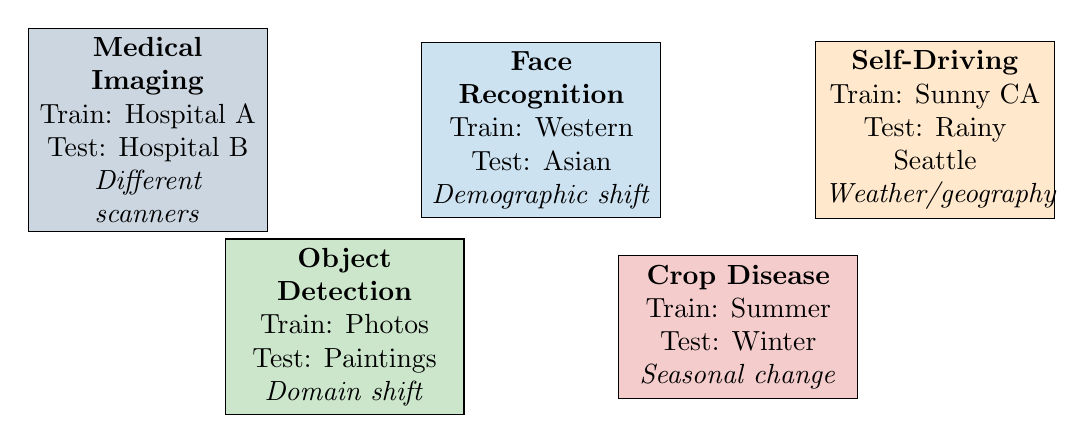
\begin{tikzpicture}[node distance=1.2cm]
    % Medical imaging
    \node[draw,rectangle,minimum width=3cm,minimum height=1.5cm,fill=ukhblue!20] (med) at (0,3) {
        \begin{minipage}{2.8cm}\centering
        \textbf{Medical Imaging}\\
        Train: Hospital A\\
        Test: Hospital B\\
        \textit{Different scanners}
        \end{minipage}
    };
    
    % Face recognition
    \node[draw,rectangle,minimum width=3cm,minimum height=1.5cm,fill=ukhlight!20] (face) at (5,3) {
        \begin{minipage}{2.8cm}\centering
        \textbf{Face Recognition}\\
        Train: Western\\
        Test: Asian\\
        \textit{Demographic shift}
        \end{minipage}
    };
    
    % Autonomous driving
    \node[draw,rectangle,minimum width=3cm,minimum height=1.5cm,fill=warningorange!20] (auto) at (10,3) {
        \begin{minipage}{2.8cm}\centering
        \textbf{Self-Driving}\\
        Train: Sunny CA\\
        Test: Rainy Seattle\\
        \textit{Weather/geography}
        \end{minipage}
    };
    
    % Object detection
    \node[draw,rectangle,minimum width=3cm,minimum height=1.5cm,fill=successgreen!20] (obj) at (2.5,0.5) {
        \begin{minipage}{2.8cm}\centering
        \textbf{Object Detection}\\
        Train: Photos\\
        Test: Paintings\\
        \textit{Domain shift}
        \end{minipage}
    };
    
    % Agricultural
    \node[draw,rectangle,minimum width=3cm,minimum height=1.5cm,fill=alertred!20] (agri) at (7.5,0.5) {
        \begin{minipage}{2.8cm}\centering
        \textbf{Crop Disease}\\
        Train: Summer\\
        Test: Winter\\
        \textit{Seasonal change}
        \end{minipage}
    };
\end{tikzpicture}
\end{center}

\textbf{Common theme:} Training data doesn't capture full real-world variability.
\end{frame}

\begin{frame}{Case Study: ImageNet to Real-World Deployment}

\textbf{ImageNet (Lab):} 96\%+ accuracy achieved!

\vspace{0.5em}

\textbf{Real-World Deployment (Factory floor):}
\begin{itemize}
    \setlength{\itemsep}{0.2em}
    \small
    \item Factory: 60\% accuracy
    \item Hospital: 45\% accuracy
    \item User photos: 70\% accuracy
\end{itemize}

\vspace{0.6em}

\textbf{Why the gap?}
\begin{itemize}
    \setlength{\itemsep}{0.2em}
    \small
    \item ImageNet: clean, centered, well-lit objects
    \item Real world: blur, weird angles, poor lighting
    \item Geographic bias: 45\% of ImageNet from USA
\end{itemize}

\vspace{0.6em}

\textbf{\textcolor{alertred}{Key lesson:}} High accuracy on test data $\neq$ real-world success. Distribution shift is real.
\end{frame}

\begin{frame}{Mitigating Distribution Shift: Practical Solutions}
\small
\textbf{Problem:} Model works in lab, fails in real world.

\vspace{0.4em}

\textbf{Solution 1: Diverse Training Data}
\begin{itemize}
    \setlength{\itemsep}{0.15em}
    \small
    \item Collect from many angles, lighting, backgrounds
    \item Use data augmentation (rotate, flip, blur)
\end{itemize}

\vspace{0.4em}

\textbf{Solution 2: Monitor in Production}
\begin{itemize}
    \setlength{\itemsep}{0.15em}
    \small
    \item Track accuracy after deployment
    \item Retrain with new real-world data
\end{itemize}

\vspace{0.4em}

\textbf{Solution 3: Ensembles}
\begin{itemize}
    \setlength{\itemsep}{0.15em}
    \small
    \item Train on different data sources
    \item Combine predictions for robustness
\end{itemize}
\end{frame}

% ============================================================================
\section{Dataset Bias and Shortcut Learning}
% ============================================================================

\begin{frame}
\begin{center}
\Large
\textit{"Big Data is a technology of amplification. It amplifies the good, the bad, and the ugly."}\\[1em]
— Evgeny Morozov
\end{center}
\end{frame}

\begin{frame}{The Path of Least Resistance}
\begin{philosophical}
\textit{"Big Data processes codify the past. They do not invent the future."}\\
\hfill — Cathy O'Neil
\end{philosophical}

\vspace{1em}

\textbf{Neural networks are lazy learners:}
\begin{itemize}
    \item They find the \textit{easiest} pattern that minimizes loss
    \item Not necessarily the \textit{right} pattern we intended
    \item This leads to \textbf{shortcut learning}
\end{itemize}

\vspace{1em}

\textbf{Example:} "Cow" classifier
\begin{itemize}
    \item Dataset: All cow images have green grass backgrounds
    \item Network learns: green pixels $\rightarrow$ cow
    \item Fails on: cow in barn, cow in snow, grass without cow
\end{itemize}
\end{frame}

\begin{frame}{Shortcut Learning: Mechanism}
\begin{center}
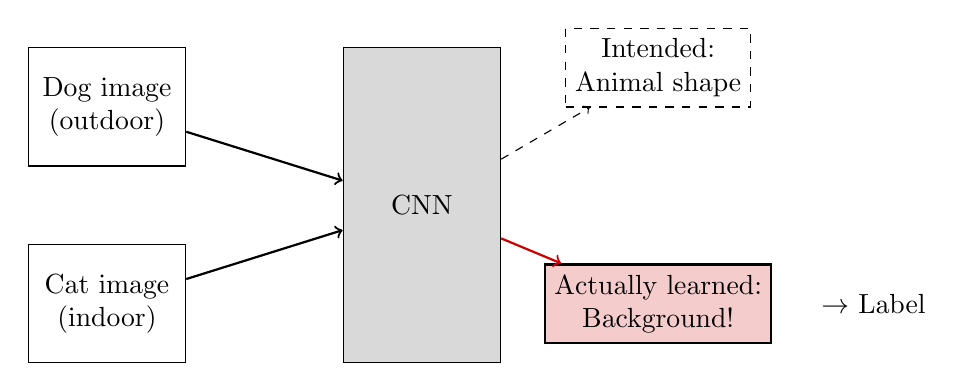
\begin{tikzpicture}[node distance=2.5cm]
    % Input images
    \node[draw,minimum width=2cm,minimum height=1.5cm,align=center] (dog) at (0,2) {Dog image\\(outdoor)};
    \node[draw,minimum width=2cm,minimum height=1.5cm,align=center] (cat) at (0,-0.5) {Cat image\\(indoor)};
    
    % Network (black box)
    \node[draw,rectangle,minimum width=2cm,minimum height=4cm,fill=gray!30] (net) at (4,0.75) {CNN};
    
    % Intended feature
    \node[draw,dashed,minimum width=2cm,minimum height=1cm,align=center] (intended) at (7,2.5) {Intended:\\Animal shape};
    
    % Actual feature
    \node[draw,thick,minimum width=2cm,minimum height=1cm,align=center,fill=alertred!20] (actual) at (7,-0.5) {Actually learned:\\Background!};
    
    % Arrows
    \draw[->,thick] (dog) -- (net);
    \draw[->,thick] (cat) -- (net);
    \draw[->,dashed] (net) -- (intended);
    \draw[->,thick,alertred] (net) -- (actual);
    
    % Label
    \node[right=0.5cm of actual] {$\rightarrow$ Label};
\end{tikzpicture}
\end{center}

\begin{warning}
If background correlates perfectly with label in training data, network has no incentive to learn the actual object!
\end{warning}
\end{frame}

\begin{frame}{Real Examples of Shortcut Learning}
\begin{enumerate}
    \item \textbf{CLEVR dataset} (reasoning task)
    \begin{itemize}
        \item Models learned to count objects by total pixel count
        \item Ignored spatial relationships entirely
    \end{itemize}
    
    \item \textbf{Pneumonia detection from X-rays}
    \begin{itemize}
        \item Model learned hospital-specific markers in images
        \item Predicted hospital, not disease!
    \end{itemize}
    
    \item \textbf{Husky vs Wolf classifier}
    \begin{itemize}
        \item Training: wolves always in snow, huskies on grass
        \item Network learned snow = wolf
        \item Saliency maps highlighted background, not animal
    \end{itemize}
    
 
    
\end{enumerate}
\end{frame}

\begin{frame}
\begin{center}
\Large
\textit{"If you don't have the data to represent a community, you don't have the data to make decisions for that community."}\\[1em]
— Timnit Gebru
\end{center}
\end{frame}

\begin{frame}{Why This Happens (The Lazy Way Out)}

\textbf{Neural networks are greedy.} They take the easiest path to minimize loss.

\vspace{1em}

\textbf{If your training data has a shortcut:}
\begin{itemize}
    \setlength{\itemsep}{0.3em}
    \item All cows have grass background $\rightarrow$ Learn grass = cow
    \item All X-rays from hospital A have a mark $\rightarrow$ Learn mark = sick
    \item Background more predictive than the object itself
\end{itemize}

\vspace{1em}

\textbf{Why does the model prefer shortcuts?}
\begin{itemize}
    \setlength{\itemsep}{0.3em}
    \small
    \item Faster to learn (fewer complex features needed)
    \item Lower loss with less effort
    \item No incentive to learn the ``right'' thing if a shortcut works
\end{itemize}

\vspace{0.8em}

\textcolor{alertred}{\textbf{The problem:}} Shortcuts work on training data but fail in the real world.
\end{frame}

\begin{frame}
\begin{center}
\Large
\textit{"Bias isn't only in people; it gets baked into datasets, then amplified by systems that scale decisions to millions."}\\[1em]
— Timnit Gebru
\end{center}
\end{frame}

\begin{frame}{Detecting Shortcuts in Your Model}

\textbf{Simple tests you can run:}

\vspace{0.8em}

\textbf{1. Mask the object, keep background}
\begin{itemize}
    \small
    \item Take the object out, show only background
    \item Model still predicts same class? $\rightarrow$ Learned the background!
\end{itemize}

\vspace{0.5em}

\textbf{2. Change the background, keep object}
\begin{itemize}
    \small
    \item Put object on different background
    \item Prediction changes? $\rightarrow$ Background matters too much
\end{itemize}

\vspace{0.5em}

\textbf{3. Look at what model focuses on}
\begin{itemize}
    \small
    \item Use visualization tools (heatmaps) to see what pixels matter
    \item Highlighting background instead of object? $\rightarrow$ Shortcut!
\end{itemize}

\vspace{0.8em}

\small \textit{Do these checks. Shortcuts are sneaky but detectable.}
\end{frame}

\begin{frame}
\begin{center}
\Large
\textit{"If your dataset has blind spots, your AI will mistake blindness for certainty."}
\end{center}
\end{frame}

\begin{frame}{Dataset Bias: Geographic and Cultural}
\begin{reality}
\small
\textbf{ImageNet:} 45\% USA, 15\% other Western, 40\% rest of world

\vspace{0.3em}

\textbf{Consequences:}
\begin{itemize}
    \setlength{\itemsep}{0.15em}
    \small
    \item "Wedding": Western white dresses dominate
    \item "Houses": Modern Western styles only
    \item Fails on traditional/regional contexts
\end{itemize}

\vspace{0.3em}

\textbf{Medical:} 85\%+ from Western hospitals — different demographics, disease patterns
\end{reality}
\end{frame}

\begin{frame}
\begin{center}
\Large
\textit{"Data doesn't describe reality; it describes what your system managed to notice."}
\end{center}
\end{frame}

\begin{frame}{Mitigating Dataset Bias and Shortcuts}

\textbf{When collecting data:}
\begin{itemize}
    \setlength{\itemsep}{0.25em}
    \small
    \item Get diverse backgrounds, lighting, angles
    \item Include different demographics and cultures
    \item Balance classes so one isn't overrepresented
\end{itemize}

\vspace{0.6em}

\textbf{When training:}
\begin{itemize}
    \setlength{\itemsep}{0.25em}
    \small
    \item Augment data: rotate, change backgrounds, vary conditions
    \item Remove obvious correlations before training
    \item Test on diverse, out-of-distribution data
\end{itemize}

\vspace{0.6em}

\textbf{Bottom line:}
\begin{itemize}
    \setlength{\itemsep}{0.25em}
    \small
    \item Your dataset bias will become your model's bias
    \item More diverse training data = more robust model
    \item Always test on data different from training
\end{itemize}
\end{frame}


% ============================================================================
\section{Overfitting and Regularization}
% ============================================================================

\begin{frame}
\begin{center}
\Large
\textit{"If you torture the data long enough, it will confess."}
\end{center}
\end{frame}

\begin{frame}{Overfitting: The Central Challenge}
\begin{center}
\Large \textbf{Overfitting = Memorization without Understanding}
\end{center}

\vspace{1em}

\textbf{Signs of overfitting:}
\begin{enumerate}
    \item Training loss $\downarrow$, validation loss $\uparrow$
    \item Training accuracy $\gg$ validation accuracy
    \item Model performs perfectly on training data
    \item Model fails on slightly different test data
\end{enumerate}

\vspace{1em}

\begin{reality}
From Chapter 11: Spiral dataset showed 98\% train accuracy vs 80\% test accuracy.\\
Gap of 18\% is severe overfitting!
\end{reality}
\end{frame}

\begin{frame}{When Does Overfitting Happen?}

\textbf{Overfitting happens when:}

\vspace{0.8em}

\textbf{1. Model is too complex}
\begin{itemize}
    \small
    \item Too many layers, too many neurons
    \item Model can memorize training data exactly
    
\end{itemize}

\vspace{0.6em}

\textbf{2. Not enough training data}
\begin{itemize}
    \small
    \item Few training examples, many model parameters
    \item Model can learn specific examples by heart
    \item Example: Deep network trained on 100 images
\end{itemize}

\vspace{0.6em}

\textbf{3. Train for too long}
\begin{itemize}
    \small
    \item Model keeps improving on training set
    \item But validation loss starts increasing
    \item Model has memorized the noise
\end{itemize}

\vspace{0.8em}

\small \textit{Real-world rule: If train accuracy is 99\% and test accuracy is 70\%, you're overfitting.}
\end{frame}

\begin{frame}{The Regularization Arsenal}

\textbf{Regularization = Preventing overfitting.}

\vspace{0.5em}

\textbf{1. L1 \& L2 Regularization}
\begin{itemize}
    \setlength{\itemsep}{0.15em}
    \small
    \item Penalize large weights in the loss function
    \item L2: weights pushed toward zero
\end{itemize}

\vspace{0.4em}

\textbf{2. Dropout}
\begin{itemize}
    \setlength{\itemsep}{0.15em}
    \small
    \item Randomly disable neurons during training
    \item Forces network to learn robust patterns
\end{itemize}

\vspace{0.4em}

\textbf{3. Early Stopping}
\begin{itemize}
    \setlength{\itemsep}{0.15em}
    \small
    \item Stop training when validation loss increases
    \item Simplest and most effective
\end{itemize}

\vspace{0.5em}

\small \textit{Use multiple techniques together for best results.}
\end{frame}

\begin{frame}{Early Stopping: The Simplest Fix}

\textbf{What is it:} Stop training when validation loss increases.

\vspace{0.6em}

\textbf{How it works:}
\begin{enumerate}
    \setlength{\itemsep}{0.2em}
    \small
    \item Monitor validation loss during training
    \item When it starts increasing, stop
    \item Use the model from the best epoch
\end{enumerate}

\vspace{0.6em}

\textbf{Why it works:}
\begin{itemize}
    \setlength{\itemsep}{0.2em}
    \small
    \item Training loss always decreases
    \item Validation loss eventually increases (memorizing noise)
    \item Stop before overfitting happens
\end{itemize}

\vspace{0.6em}

\begin{keypoint}
Early stopping is \textbf{free} — use it always. No tuning needed.
\end{keypoint}
\end{frame}

\begin{frame}{Dropout: Ensemble in One Model}

\textbf{What is it:} During training, randomly disable 50\% of neurons (typical).

\vspace{1em}

\textbf{Why it works:}
\begin{itemize}
    \setlength{\itemsep}{0.25em}
    \small
    \item Neurons can't rely on specific neighbors
    \item Forces network to learn redundant representations
    \item Makes features more robust
    \item At test time, use all neurons (learned features are reliable)
\end{itemize}

\vspace{1em}

\textbf{Simple analogy:}
\begin{itemize}
    \setlength{\itemsep}{0.25em}
    \small
    \item Like training an ensemble: each neuron learns slightly different patterns
    \item At test, combine all the diverse knowledge
    \item More robust predictions
\end{itemize}

\vspace{0.8em}

\small \textit{Dropout is especially effective in deep networks.}
\end{frame}

\begin{frame}{Putting It All Together: A Practical Strategy}
\small
\textbf{Before training:}
\begin{itemize}
    \setlength{\itemsep}{0.15em}
    \small
    \item Diverse data, simple model, add dropout
\end{itemize}

\vspace{0.3em}

\textbf{During training:}
\begin{itemize}
    \setlength{\itemsep}{0.15em}
    \small
    \item Early stopping on validation
    \item Monitor train and validation loss
\end{itemize}

\vspace{0.3em}

\textbf{After training:}
\begin{itemize}
    \setlength{\itemsep}{0.15em}
    \small
    \item Check test performance
    \item If overfitting: augment data or simplify model
\end{itemize}

\vspace{0.5em}

\small \textit{Iterative process. Test and adjust.}
\end{frame}


% ============================================================================
\section{Case Studies}
% ============================================================================

\begin{frame}{Case Study 1: Medical Imaging Disaster}
\begin{reality}
\textbf{What happened:}
\begin{itemize}
    \setlength{\itemsep}{0.15em}
    \small
    \item Train on Hospital A: 97\% accuracy
    \item Deploy to Hospital B: 62\% accuracy
\end{itemize}

\textbf{Root cause:}
\begin{itemize}
    \setlength{\itemsep}{0.15em}
    \small
    \item Model learned hospital-specific markers, not disease
    \item Different scanner = different image characteristics
\end{itemize}
\end{reality}
\end{frame}

\begin{frame}{Case Study 1: Lessons Learned}

\textbf{What went wrong:}
\begin{itemize}
    \setlength{\itemsep}{0.2em}
    \small
    \item No external validation from different hospital
    \item Didn't visualize what model learned
    \item Train/test from same source only
\end{itemize}

\vspace{0.5em}

\textbf{The Fix:}
\begin{itemize}
    \setlength{\itemsep}{0.2em}
    \small
    \item Collect from multiple hospitals
    \item Validate on different institutions
    \item Visualize model focus (saliency maps)
\end{itemize}

\vspace{0.8em}

\small \textit{Lesson: High test accuracy $\neq$ real-world success. Validate on target domain.}
\end{frame}

\begin{frame}{Case Study 2: License Plate Recognition}
\begin{reality}
\textbf{Setup:} Train on European plates (99\% accurate) $\rightarrow$ Deploy in Kurdistan (45\% accurate)

\vspace{0.5em}

\textbf{Problems:}
\begin{itemize}
    \setlength{\itemsep}{0.15em}
    \small
    \item Different fonts, sizes, colors, Arabic numerals
    \item Training $\neq$ deployment distribution
\end{itemize}
\end{reality}
\end{frame}

\begin{frame}{Case Study 2: Recovery Strategy}

\textbf{What to do:}
\begin{itemize}
    \setlength{\itemsep}{0.2em}
    \small
    \item Collect local data + fine-tune (accuracy: 45\% $\rightarrow$ 85\%)
    \item Build diverse training from the start
    \item Include international variants
    \item Test on data from different regions
\end{itemize}

\vspace{0.8em}

\textbf{Key lesson:}
\begin{itemize}
    \setlength{\itemsep}{0.2em}
    \small
    \item Don't assume deployment = training distribution
    \item Always validate cross-domain generalization
    \item Real-world is messier than your benchmark
\end{itemize}
\end{frame}

\begin{frame}{Case Study 3: ImageNet Overconfidence}
\small
\textbf{Problem:} ResNet-50 overconfident on new data

\vspace{0.5em}

\textbf{Results:}
\begin{itemize}
    \setlength{\itemsep}{0.15em}
    \small
    \item ImageNet: 96\% accuracy
    \item New images: 84\%, Corrupted: 60\%
    \item Wrong predictions often >90\% confident!
\end{itemize}

\vspace{0.5em}

\textbf{Lesson:} Model doesn't know what it doesn't know. Use calibration techniques:
\begin{itemize}
    \item Temperature scaling
    \item Ensemble methods
    \item Bayesian neural networks for uncertainty
\end{itemize}
\end{frame}


% ============================================================================
\section{Practical Checklist and Best Practices}
% ============================================================================

\begin{frame}{The Honest Evaluation Checklist}
\small
\textbf{Before claiming your model works:}

\vspace{0.4em}

\textbf{Data:}
\begin{itemize}
    \setlength{\itemsep}{0.15em}
    \small
    \item \checkmark Splits defined before any processing (no leakage)
    \item \checkmark Preprocessing fitted only on training data
\end{itemize}

\textbf{Evaluation:}
\begin{itemize}
    \setlength{\itemsep}{0.15em}
    \small
    \item \checkmark Metrics appropriate for class balance
    \item \checkmark Hyperparameters tuned on validation, not test
    \item \checkmark Test set evaluated only once at the end
    \item \checkmark Baseline comparisons included
\end{itemize}

\textbf{Transparency:}
\begin{itemize}
    \setlength{\itemsep}{0.15em}
    \small
    \item \checkmark Learning curves show no overfitting
    \item \checkmark Failure cases analyzed
\end{itemize}
\end{frame}

\begin{frame}{Red Flags: Something's Wrong}
\small
\textbf{Be suspicious if you see:}

\vspace{0.4em}

\begin{itemize}
    \setlength{\itemsep}{0.2em}
    \small
    \item \texttimes\ Test accuracy = 99.9\% (too perfect, probably leakage)
    \item \texttimes\ Train and test within 0.1\% (definite leakage!)
    \item \texttimes\ No validation set mentioned
    \item \texttimes\ Multiple "final" test evaluations
    \item \texttimes\ Performance beats strong baselines by huge margin
    \item \texttimes\ No failure analysis or limitations
\end{itemize}

\vspace{0.5em}

\begin{warning}
\small
If it looks too good to be true, it probably is. Dig deeper!
\end{warning}
\end{frame}

\begin{frame}{Publication Best Practices}
\textbf{When publishing ML research, report:}

\begin{enumerate}
    \item \textbf{Dataset details:} Size, split, collection procedure
    \item \textbf{Preprocessing:} Every step, in order
    \item \textbf{Architecture:} Complete specification
    \item \textbf{Hyperparameters:} All of them, including those "not tuned"
    \item \textbf{Training details:} Optimizer, learning rate schedule, epochs, hardware
    \item \textbf{Multiple metrics:} Accuracy, F1, AUC, etc.
    \item \textbf{Confidence intervals:} Via bootstrap or multiple runs
    \item \textbf{Baseline comparisons:} Fair, controlled comparisons
    \item \textbf{Ablation studies:} What components matter?
    \item \textbf{Failure analysis:} Where does model fail and why?
\end{enumerate}

\vspace{0.5em}

\textbf{Goal:} Reproducibility and intellectual honesty.
\end{frame}

\begin{frame}{Common Mistakes to Avoid}
\small

\textbf{Don't do these:}

\vspace{0.3em}

\begin{enumerate}
    \setlength{\itemsep}{0.2em}
    \small
    \item Tuning on test set \texttimes\ (invalidates everything)
    \item Ignoring class imbalance (accuracy misleads)
    \item No external validation (overly optimistic)
    \item Cherry-picking metrics (confirmation bias)
    \item Not checking for shortcuts (learns wrong patterns)
    \item Claiming causation from correlation
    \item Comparing unfairly (different splits/preprocessing)
    \item Forgetting deployment reality (lab $\neq$ real world)
\end{enumerate}
\end{frame}

% ============================================================================
\section{Philosophical Reflections and Future}
% ============================================================================

\begin{frame}
\begin{center}
\Large
\textit{"Whoever owns the data often writes the future in advance."}
\end{center}
\end{frame}

\begin{frame}{What Are We Really Building?}
\begin{philosophical}
\textit{"Technology is never neutral. Every algorithm encodes a worldview, and every dataset reflects a history."}\\
\hfill — Paraphrased from critical AI studies
\end{philosophical}

\vspace{1em}

\textbf{Our models reveal:}
\begin{itemize}
    \item What data we had access to (privilege)
    \item What patterns we chose to encode (values)
    \item What errors we tolerate (priorities)
    \item Who we included and excluded (power)
\end{itemize}

\vspace{1em}

\textbf{Generalization is not just technical:}
\begin{itemize}
    \item Whose reality does our model generalize to?
    \item Who benefits? Who is harmed?
    \item What assumptions are we baking in?
\end{itemize}
\end{frame}

\begin{frame}{The Myth of Objective Data}
\begin{philosophical}
\textit{"Data is not raw truth — it is collected, curated, and cleaned by humans with specific goals and biases."}\\
\end{philosophical}

\vspace{1em}

\textbf{Every dataset embeds choices:}
\begin{itemize}
    \item What to include (and exclude)
    \item How to label (and by whom)
    \item What quality standards to apply
    \item What context to preserve or discard
\end{itemize}

\vspace{1em}


\end{frame}

\begin{frame}{From Patterns to Wisdom}
\begin{philosophical}
\textit{"In the 21st century, the real challenge is not accessing information, but knowing what information to trust, and what to ignore."}\\
\hfill — Yuval Noah Harari, \textit{Nexus}
\end{philosophical}

\vspace{1em}

\textbf{The generalization hierarchy:}
\begin{enumerate}
    \item \textbf{Data:} Raw observations (pixels, measurements)
    \item \textbf{Information:} Structured patterns (features, correlations)
    \item \textbf{Knowledge:} Validated models (functions that generalize)
    \item \textbf{Wisdom:} Understanding limitations and context
\end{enumerate}

\vspace{1em}

\textbf{Our responsibility:} Move from building models that \textit{memorize} to models that \textit{understand}, while acknowledging they will never fully reach human wisdom.
\end{frame}

\begin{frame}{The Future of Generalization}
\textbf{Emerging challenges:}
\begin{itemize}
    \item \textbf{Multi-modal models:} Generalizing across vision, language, audio
    \item \textbf{Foundation models:} Pre-trained on massive data, fine-tuned everywhere
    \item \textbf{Continual learning:} Models that adapt without forgetting
    \item \textbf{Few-shot generalization:} Learning from minimal examples
    \item \textbf{Robustness to adversarial attacks:} Worst-case generalization
\end{itemize}

\vspace{1em}

\textbf{Open questions:}
\begin{itemize}
    \item Can we build models that generalize like humans?
    \item How to quantify and guarantee safety under distribution shift?
    \item How to make generalization fair across all demographics?
    \item What are the fundamental limits of generalization?
\end{itemize}
\end{frame}

% ============================================================================
\section{Summary and Key Takeaways}
% ============================================================================

\begin{frame}{Key Messages: Part I — Foundations}
\begin{enumerate}
    \item \textbf{Generalization is the only thing that matters.} Training performance is a means, not an end.
    
    \item \textbf{Neural networks are powerful memorizers.} They will take the path of least resistance — our job is to guide them toward understanding, not memorization.
    
    \item \textbf{Data splitting is fundamental.} Train/Val/Test must be carefully designed to prevent leakage and reflect real-world deployment.
    
    \item \textbf{IID assumption is usually violated.} Distribution shift is the norm, not the exception.
\end{enumerate}
\end{frame}

\begin{frame}{Key Messages: Part II — Evaluation}
\begin{enumerate}
    \setcounter{enumi}{4}
    \item \textbf{Accuracy is often the wrong metric.} Use precision, recall, F1, AUC based on your application and class balance.
    
    \item \textbf{Every metric has uncertainty.} Report confidence intervals, not just point estimates.
    
    \item \textbf{Bias-variance tradeoff is real.} Finding the sweet spot between underfitting and overfitting is an art.
    
    \item \textbf{Shortcuts are everywhere.} Models learn easiest patterns, which may be spurious correlations, not causal relationships.
\end{enumerate}
\end{frame}

\begin{frame}{Key Messages: Part III — Robustness}
\begin{enumerate}
    \setcounter{enumi}{8}
    \item \textbf{Regularization is essential.} L2, dropout, data augmentation, early stopping — use them all.
    
    \item \textbf{Data augmentation is the CV superpower.} Often provides bigger gains than architectural tricks.
    
    \item \textbf{External validation is critical.} Test on data from different domains, demographics, institutions.
    
    \item \textbf{Models don't know what they don't know.} Calibration and OOD detection are necessary for safe deployment.
\end{enumerate}
\end{frame}

\begin{frame}{The Philosophical Core}
\begin{philosophical}
\textit{"The question is not whether our neural networks can learn patterns — they excel at that. The question is whether they learn the right patterns, whether they generalize fairly, and whether we understand their limitations well enough to deploy them responsibly."}
\end{philosophical}

\vspace{1em}

\textbf{As future AI practitioners:}
\begin{itemize}
    \item We are not just data scientists — we are architects of decision-making systems
    \item Our models' failures reveal what we value and who we exclude
    \item Generalization is not just technical — it's ethical, social, political
    \item We must build systems with humility, acknowledging what we cannot know
\end{itemize}
\end{frame}

\begin{frame}{Final Reflection}
\begin{philosophical}
\textit{"Technology isn't a window onto the world—it's a mirror. What we see reflects not objective reality, but the choices, biases, and values we encoded into our systems."}\\
\hfill Yuval Noah Harari, \textit{Nexus}
\end{philosophical}

\vspace{1em}

\textbf{Your mission:}
\begin{itemize}
    \item Build models that generalize \textit{fairly} across all populations
    \item Question assumptions embedded in datasets
    \item Report limitations honestly
    \item Advocate for diverse, representative data
    \item Never deploy without rigorous out-of-sample testing
\end{itemize}

\vspace{0.2em}

The future of AI depends not just on better algorithms, but on better \textit{evaluation culture} — one that prioritizes honesty, robustness, and equity.
\end{frame}

% ============================================================================
\section{References}
% ============================================================================

\begin{frame}{References — Books and Foundational Texts}
\begin{thebibliography}{99}
\footnotesize

\bibitem{nnfs}
Harrison Kinsley \& Daniel Kukieła (2020).
\textit{Neural Networks from Scratch in Python}.
Self-published. Chapter 11: Testing with Out-of-Sample Data.

\bibitem{goodfellow}
Ian Goodfellow, Yoshua Bengio, Aaron Courville (2016).
\textit{Deep Learning}.
MIT Press. Chapter 5 (Machine Learning Basics), Chapter 7 (Regularization).

\bibitem{harari_deus}
Yuval Noah Harari (2016).
\textit{Homo Deus: A Brief History of Tomorrow}.
Harper. Discussions on data, information, and algorithms.

\bibitem{harari_nexus}
Yuval Noah Harari (2024).
\textit{Nexus: A Brief History of Information Networks from the Stone Age to AI}.
Random House. Perspectives on information, trust, and AI systems.

\bibitem{bishop}
Christopher M. Bishop (2006).
\textit{Pattern Recognition and Machine Learning}.
Springer. Chapter 1 (Introduction), Chapter 3 (Linear Models).

\end{thebibliography}
\end{frame}

\begin{frame}{References — Research Papers (1/2)}
\begin{thebibliography}{99}
\footnotesize

\bibitem{vapnik}
Vladimir Vapnik (1999).
\textit{The Nature of Statistical Learning Theory} (2nd ed.).
Springer. VC dimension and generalization bounds.

\bibitem{understanding}
Chiyuan Zhang et al. (2017).
``Understanding deep learning requires rethinking generalization.''
ICLR 2017.

\bibitem{shortcuts}
Robert Geirhos et al. (2020).
``Shortcut learning in deep neural networks.''
\textit{Nature Machine Intelligence}, 2, 665–673.

\bibitem{imagenet_bias}
Kaiyu Yang \& Olga Russakovsky (2020).
``A study of face obfuscation in ImageNet.''
ICML 2020.

\bibitem{distribution_shift}
Joaquin Quiñonero-Candela et al. (2009).
\textit{Dataset Shift in Machine Learning}.
MIT Press.

\end{thebibliography}
\end{frame}

\begin{frame}{References — Research Papers (2/2)}
\begin{thebibliography}{99}
\footnotesize

\bibitem{mixup}
Hongyi Zhang et al. (2018).
``mixup: Beyond Empirical Risk Minimization.''
ICLR 2018.

\bibitem{cutmix}
Sangdoo Yun et al. (2019).
``CutMix: Regularization Strategy to Train Strong Classifiers with Localizable Features.''
ICCV 2019.

\bibitem{calibration}
Chuan Guo et al. (2017).
``On Calibration of Modern Neural Networks.''
ICML 2017.

\bibitem{dropout}
Nitish Srivastava et al. (2014).
``Dropout: A Simple Way to Prevent Neural Networks from Overfitting.''
\textit{Journal of Machine Learning Research}, 15, 1929–1958.

\bibitem{batchnorm}
Sergey Ioffe \& Christian Szegedy (2015).
``Batch Normalization: Accelerating Deep Network Training by Reducing Internal Covariate Shift.''
ICML 2015.

\end{thebibliography}
\end{frame}

\begin{frame}{References — Online Resources and Tools}
\begin{thebibliography}{99}
\footnotesize

\bibitem{sklearn_metrics}
scikit-learn documentation:
\texttt{sklearn.metrics} module.
\url{https://scikit-learn.org/stable/modules/model_evaluation.html}

\bibitem{pytorch_docs}
PyTorch documentation: Model evaluation and best practices.
\url{https://pytorch.org/tutorials/}

\bibitem{distill}
Distill.pub: Interactive visualizations of ML concepts.
\url{https://distill.pub/}

\bibitem{paperswithcode}
Papers With Code: Leaderboards and reproducibility.
\url{https://paperswithcode.com/}

\bibitem{ml_glossary}
Google's Machine Learning Glossary: Comprehensive definitions.
\url{https://developers.google.com/machine-learning/glossary}

\end{thebibliography}
\end{frame}

% ============================================================================
\section*{Closing}
% ============================================================================

\begin{frame}{Thank You}
\begin{center}
{\Large \textbf{Questions or Discussion?}}

\vspace{2em}

\begin{tabular}{rl}
\textbf{Student:} & Davar Adil Yassin \\
\textbf{Institution:} & University of Kurdistan Hewlêr (UKH) \\
\textbf{Program:} & MSc in Artificial Intelligence \\
\textbf{Course:} & Computer Vision \\
\textbf{Instructor:} & Dr. Polla \\
\textbf{Date:} & 16 December 2025 \\
\end{tabular}

\vspace{2em}

\textit{Remember: The goal is not just to build models that work,\\
but to build models that work \textbf{for everyone}, \textbf{fairly}, and \textbf{transparently}.}
\end{center}
\end{frame}
\end{document}